% Created 2019-12-14 Sat 23:41
% Intended LaTeX compiler: pdflatex
\documentclass[11pt]{article}
\usepackage[utf8]{inputenc}
\usepackage[T1]{fontenc}
\usepackage{graphicx}
\usepackage{grffile}
\usepackage{longtable}
\usepackage{wrapfig}
\usepackage{rotating}
\usepackage[normalem]{ulem}
\usepackage{amsmath}
\usepackage{textcomp}
\usepackage{amssymb}
\usepackage{capt-of}
\usepackage{hyperref}
\usepackage{minted}
\usepackage[margin=.5in]{geometry}
\renewcommand{\familydefault}{\sfdefault}
\author{Guilherme Gomes Haetinger}
\date{\emph{University of California, Berkeley} \\ Fall 2019 \\ - \emph{Share this with whomever you want. If you spot a mistake, email me at ghaetinger@gmail.com} -}
\title{\huge Computer Security - Semester Review}
\hypersetup{
 pdfauthor={Guilherme Gomes Haetinger},
 pdftitle={\huge Computer Security - Semester Review},
 pdfkeywords={},
 pdfsubject={},
 pdfcreator={Emacs 27.0.50 (Org mode 9.2.6)}, 
 pdflang={English}}
\begin{document}

\maketitle
\tableofcontents


\section{Security Design}
\label{sec:orgf13f6e5}
Let's discuss on how to make a system theoretically secure, as in the decisions that should be made and what are the main points we should leverage when designing a system from scratch. 
\subsection{Security Principles}
\label{sec:org4ab8166}
We have a number of security principles that must be considered once we are developing software \cite{wagner_security_2019}. Some of them can be enumerated as the most important. These are:
\begin{itemize}
\item \textbf{Security is Economics}: Only spend as much money as what you are trying protect is worth. \uline{Don't buy a \$10000 lock for a \$10 bike}.
\item \textbf{Least Privilege}: Only give a program the actual amount of privilege it needs to do its purpose. \uline{We should not give ROOT access to a program that plays the nyan cat video}.
\item \textbf{Fail-safe Defaults}: Safe defaults in the sense of "\emph{if something fails, what should be the current state?}". It's recommended that we use \emph{default-deny} policies. \uline{The light goes down on a server's building. Should the electronic lock on the server access door be unlocked or stay locked?} \(\to\) If we want \emph{default-deny} policies, the door will stay shut, keeping the server's hardware safe from whomever wants to access it, which will keep it secure from someone who jammed the building's circuits just to get to the computers.
\item \textbf{Separation of Responsibility}: Separate privilege. "Nobody has full privilege by itself". \uline{Nuke triggers need multiple people turning a key to work (at least in movies)}.
\item \textbf{Defense in Depth}: Create redundant layers of protection. \uline{In the medieval times, castles were protected by an outer wall and an inner wall, so that enemies would have to go through 2 different walls to truly invade it. This made the process much harder}.
\item \textbf{Psychological Acceptability}: "Users must buy into your security model". If you want users to use your safety resources, make it easy to do so. \uline{If to process a company transaction, the user is asked to fill a form of 100 pages, after processing a number of transactions, the user will tire and just leave the form aside, hoping that nobody checks it}.
\item \textbf{Human Factors}: Always consider human factors. Things must be usable. Don't make it hard for an ordinary user to interact with your system. \uline{Don't make regular users think of a password with 15 different upper case letters, all the letters in the alphabet and at least 5 letters of the ancient Greek alphabet}.
\item \textbf{Complete Mediation}: Make sure you have control over \textbf{every} point of access. Enforce access control policies. \uline{Bottleneck the airport's immigration procedural check so you know every immigrant is treated the same controlled way}.
\item \textbf{Know your threat model}: Consider changes in your threat model. Keep track of it and ensure you are safe from it. \uline{Internet was made for researches with no threat model whatsoever. When they opened for the public, they had to consider the malicious use of the internet. It now had a threat model}.
\item \textbf{Don't rely on Security through Obscurity}: Don't rely on the fact that your design/algorithm is secret. \uline{You design a code that sends the user's password unencrypted back to the server for some weird reason. You provide your system as compiled code, in a way that the user can't interpret it correctly. The user may be able to reverse engineer it and hijack the server connection to get other user's passwords}.
\item \textbf{Design Security from the start}: Don't leave security out for refactoring. It's usually really difficult to refactor code in order to make it secure because it needs a system redesign. \uline{A webpage has users and their given passwords. They allowed whatever password the user wanted to use on it. They decide to restrain to safer 16-character passwords with all the right shenanigans. What happens to the already created accounts? Do you make them redo their password, which should take a lot of time? Or do you maintain them unsafe?}.
\item \textbf{Kerkchoff's Principle}: Similar to the \emph{Don't rely on Security through Obscurity} principle, this one asks you to "Design your system as if the attacker could read your code". We can consider the same example as the referred principle.
\end{itemize}
\subsection{Security Design Patterns \& What you should think about when designing your system}
\label{sec:org3a2ed56}
How should we go at \emph{Developing your own secure system}?
\subsubsection{Trusted Computing Base - the \textbf{TCB}}
\label{sec:org8c470d6}
The simpler definition for this abstraction would be \emph{the part of the system in which we rely so that it works properly}, meaning that no problem outside of this part can obliterate your service. Now, the point of this design is to minimize it so that it is easier for us to place our trust in it. \uline{It's easier to place your trust in a 10 line code than in a 100.000 line code}. We want the \textbf{TCB} to be \emph{unbypassable}, \emph{tamper-resistant}, \emph{verifiable}. It is called a \emph{primitive yet effective kind of modularity}.
\subsubsection{Modularity and Isolation}
\label{sec:orgaad34ec}
The whole idea of modularity can impact on different levels of the system. Sometimes it can bring efficiency by assuming that each module already has it's own required data to run correctly. It can also provide legibility since we can understand how the code is divided into multiple responsibilities, which can impact on refactoring (can eventually help quick security patches). Now, most importantly, modularity can provide us with \emph{isolation}, meaning that each module is independent and can keep its problems to itself \(\to\) minimizes assumptions made by other components that it interacts with, enabling them to treat errors in the system without crashing it (understand what happened to the other component and act accordingly).

\section{System Implementation Vulnerabilities}
\label{sec:orgc350918}
What are the main system threats regarding its code implementation? Let's see how we can generally exploit and fix these vulnerabilities.
\subsection{Time-of-Check To Time-of-Use (TOCTTOU)}
\label{sec:org8e36a1e}
This is a general vulnerability (when I write general I mean it can happen in any logical programming environment (when I say environment I mostly mean language (when I say language it's just because Weaver specifically tells us not to use C))). As the title already says, this vulnerability takes into account the time of check for a variable and the time you assign its value. Take a look at the following code:

\begin{minted}[,bgcolor=yellow]{ruby}
def openFileOfSize200(size, filename)
  if metadata(filename).size > 200
    print "Haha this is unbypassable"
    exit
  end
  # Sleep a bit because there is definitely another process that needs CPU more than I
  sleep(1000)
  read(filename, 'r')
end
\end{minted}

This code has a flaw. As you can see, its purpose is to only read files that have the size less or equal to 200. The code reads the file metadata and checks it size. If it's bigger than the purposed value, it exits. \uline{What if I changed the file size while the program sleeps? \(\to\) The file with the larger size is read in the end, because the time of check, which is when the if-statement is run, for being far away from the time of use, enables us to bypass the check}.

\subsection{The Stack \& How C breaks it (Memory Safety)}
\label{sec:org7840f81}
Before you read anything from this section, take a look at the Appendix section on \hyperref[sec:Assemble]{Assembly code}! There is a lot of review on it needed for this part of the content. Now that that's out of the way, let's smash the stack.
\subsubsection{Format String Vulnerability}
\label{sec:orgec36168}
  For this exploit, it \textbf{very} important to understand the layout of variables inside the stack. For this, see the \hyperref[sec:VarLayoutStack]{appendix notes} on it.
We're all very familiar with \texttt{printf}. It can take \emph{1 to n} arguments, being the first a string with \textbf{hotkeys} such as \texttt{\%d, \%c, \%f, \%s, ...}. These keys represent the format of representation of a given argument. If someone just prints out user input with \texttt{printf}, the formatting string (the one with hotkeys) will be determined by the user, meaning that it can use whatever formatting string. \uline{What can a user do with its arbitrary formatting string, when the number of arguments given to printf is smaller than the number of hotkeys?}. Considering the structure of the stack when \texttt{printf} is called, the hotkeys will make the function look for a specific argument that doesn't exist, which will make it interpret whatever is in the Stack in argument's position as the one itself. The following example might clear up what I'm passing on:

\begin{minted}[]{c}
int main() {
  int num = 100;
  char buf[10];
  if(fgets(buf, sizeof buf, stdin) == NULL) return 0;
  printf(buf);
}
\end{minted}

If we use the input \texttt{\%s\%d}, we'll get the value of \texttt{buf} followed by the value of \texttt{num}. This happens because the argument that we seek to fill \texttt{\%s} will be the first memory slot above the formatting string argument and, since there are no other arguments, it will fall on the local variables of the \texttt{main} function. Hence, \texttt{\%d} will take the value of \texttt{num}, which was declared right above \texttt{buf}. \uline{Now what would we use this for?} Maybe getting the internal state of the program might be interesting for your exploit (emphasis on \textbf{Stack Canaries}).

There is another way to approach this exploit by using a specific hotkey that enables you to write the value of printed characters (until it's called) in some memory address. This hotkey is \texttt{\%n}. We can do something like this to exploit the same code but with \texttt{buf} declared before \texttt{num}. Given a number \emph{z}, we can store \emph{z} in an arbitrary address \emph{a} by inputting the following string: \texttt{a\%(z-4)x\%n}. The \texttt{printf} function will print the 4-byte address, followed by a (z-4)-byte word format of \texttt{num}, which is the last pushed local variable, and, finally, will read the first 4 bytes of \texttt{buf}, which happen to be \emph{a}, and use it as input for \texttt{\%n}, storing \(z - 4 + 4\) in \emph{a}.  

This vulnerability is easily fixed by calling \texttt{printf("\%s", buf)} instead of \texttt{printf(buf)}.
\subsubsection{Integer Conversion \& Overflow Vulnerabilities}
\label{sec:org7d2574c}
This is a simple vulnerability. Always check the type of your input as you use it in other functions. Be careful because negative \texttt{int} values can be less than whatever size check you have in your code but be extremely big when converted to \texttt{unsigned} types that are used in standard writing functions such as \texttt{memcpy}.

Also, be careful when using arithmetic operations when trying to allocate the correct amount of space for a variable. Values can overflow and allocate a much smaller memory chunk for that variable, allowing a sizable input to overflow your small sized buffer.
\subsubsection{General Protection Against Memory Attacks}
\label{sec:orge41b872}
\begin{itemize}
\item Secure code Practices
\begin{itemize}
\item Check validity of variables (not \texttt{NULL}, within bounds, \ldots{})
\item Use standard safe functions such as \texttt{strlcpy} instead of \texttt{strcpy} and \texttt{fgets} instead of \texttt{gets}
\end{itemize}
\item Using a memory-safe language
\item Runtime checking
\begin{itemize}
\item Preconditions and Post-conditions
\end{itemize}
\item Compiler's static analysis
\item Testing
\begin{itemize}
\item Test generation, Bug detection
\item Random, mutated and \emph{structure-driven} inputs.
\end{itemize}
\end{itemize}

\subsubsection{Buffer Overflow}
\label{sec:org36196d8}
This is the easiest vulnerability we were able to exploit in this class. As a trade-off of being easy to exploit, it is also easy to fix.

Given a program in a language that doesn't implement memory safety (C), we can have programs that for a given input behave maliciously. We can do this via the \emph{Buffer Overflow} vulnerability in some programs. This is, nonetheless, the ability of filling a variable with a value that doesn't fit in it, enabling us to write on the memory that is above it in the Stack. For example:

\begin{minted}[,bgcolor=yellow]{c}
int main() {
  char input[4];
  gets(input);
  return 0;
}
\end{minted}

We know that \texttt{gets} reads whatever you input and writes it into a variable with a \texttt{'\textbackslash{}0'} in the end. \uline{What happens if we input the output of the following python code in it?}

\begin{minted}[,bgcolor=yellow]{python}
print("a"*4 + "b"*4 + address_for_malicious_code)
\end{minted}

What happens is (considering no callee registers):
\begin{itemize}
\item The variable \texttt{input} will have been filled up by \texttt{"a"s};
\item The \texttt{EBP} value will have been filled up by \texttt{"b"s};
\item The \emph{return address} will have the value of the address pointing to a malicious code (We probably should input the malicious code as well, but that would involve calculating the actual address of the variable \texttt{input}).
\end{itemize}

In the end, our stack would have the following layout:

\begin{center}
\begin{tabular}{l|l|l}
\hline
LOWEST Mem Addr. & ESP & 4 bytes\\
\hline
"input" & 4 bytes & \\
\hline
EBP & 4 bytes & \\
\hline
Return Address & 4 bytes & \\
\hline
\ldots{} &  & \\
\hline
HIGHEST Mem Addr. &  & \\
\hline
\end{tabular}
\end{center}

We can also use this to change variables that are on top of the input variables.

\subsubsection{Stack Smashing Mitigation}
\label{sec:org8b0380f}
This is a more dense subject. Considering that buffer overflow is one of the most common exploits, the following mitigation options are more complex and are harder to barge through \cite{MemoryDefenseSlide}.

\begin{enumerate}
\item \textbf{Stack Canaries}
\label{sec:org1d55b12}

Random value generated when program starts that is stored below the \texttt{EBP}. Its value is checked once the function returns and, if it has changed, the program will know it has been hijacked. The idea behind it is to avoid simple Buffer Overflows to change the value of the \texttt{EBP} or the \emph{return address}. \uline{How can we go around this mitigation?} We have to find a way \emph{not to kill the Canary}. For this, we have the following options :
\begin{itemize}
\item Find out the value of the canary and rewrite it in the process of modifying the \texttt{EBP} or \emph{return address}. To do that we either have to find a string formatting vulnerability that may print the value or any other information leak that might dump it, e.g. finding a way for the program not to read a \texttt{'\textbackslash{}0'} character in the end of a string while printing it out will make the program leak every information until the next \texttt{'\textbackslash{}0'}. The example can be easily prevented by making the first bytes of the canary always be equivalent to the end-string character, making it stop before reading the canary. While this is effective against this attack, we can see that the entropy of the canary is lowered by 25\%, which is supposed to make brute-force plausible since we now have 24 bits of entropy.
\item Use a string formatting vulnerability to write around it with specific addresses.
\end{itemize}

\item \textbf{Non-executable pages}
\label{sec:org9f26834}

We maintain the permission of writing and executing in a \texttt{XOR} condition, meaning that the program can either write code on stack/heap or execute it. This is insufficient since it is easily breakable by \textbf{Return Oriented Programming}, which is basically changing the return addresses of the code to known portions of standard libraries or even the code itself, i.e. using already written code as modules for writing your own malicious execution.

\item \textbf{Address Space Layout Randomization}
\label{sec:orgc9f2ef4}

Consists on rearranging/relocating the chunks of memory into different addresses. This makes things much harder to exploit considering that we don't have fixed addresses to write code and then redirect the execution to it. Together with \textbf{Non-executable pages}, requires an information leak to be broken. \uline{How can we bypass this?} There are some ways we can do it, but require really specific scenarios \cite{muller_aslr_nodate} and are probably not worth getting into.
\end{enumerate}

\section{Cryptography}
\label{sec:org36aa796}
Cryptography is the field of studies and implementations regarding algorithms and systems that seek to ensure \textbf{Confidentiality} (Prevent others from reading our data without authorization), \textbf{Integrity} (Prevent others from modifying our data without authorization) and \textbf{Authentication} (Asserting the identity of someone who sent a message, edited a file, etc.) to our private data. Weaver clearly emphasizes the fact that these systems are not meant to be redesigned by us because they are really easy to screw up. We'll keep using message sending as our example for every algorithm.
\subsection{Independence under Chosen Plain-Text Attack Game (IND-CPA)}
\label{sec:org9672fd9}
The IND-CPA game is designed to check whether the algorithm in question is not deterministic and, thus, is a step closer to safety. It consists of the following steps:
\begin{itemize}
\item Attacker sends two messages to an \emph{Oracle} (Entity that encrypts the messages using the encryption algorithm being tested and the \emph{K} key unknown to the Attacker);
\item \emph{Oracle} replies the encryption of one of them;
\item Attacker can do this for any message it wants as many times as it needs;
\item If Attacker has, at any point, more than 50\% chance of guessing which message was encrypted, it wins the game.
\end{itemize}

If the Attacker wins the game, we can assume that the output of the encryption algorithm can be predicted by its input even without knowing \emph{K}. This makes the algorithm extremely flawed because someone eavesdropping an encrypted conversation might be able to deterministically understand and hijack it. Therefore we seek the algorithms that win it.  
\subsection{Symmetric Encryption}
\label{sec:orgedc523e}
Given that two people (A, B) have a secret key \emph{K} known only by them. Consider \(E_K(M)\) as the encryption function and \(D_K(C)\) as the Decryption function (\(M\) is the message and \(C\) is the cypher).\cite{weaver_symmetric_nodate,symEnc,SymEncSlide}   
\subsubsection{One Time Pad}
\label{sec:orgb9f45e3}
This is the most simple encryption algorithm we saw. The calculations are self-explaining.

\begin{align*}
C &= E_K(M) = M \oplus K \\
M &= D_K(C) = C \oplus K
\end{align*}

It's trivial to understand why this is a IND-CPA loser. This example shows why

\begin{align}
A &\to_{M1,M2} O \\
O &: C1 = M2 \oplus K \\
O &\to_{C1}_{}_{} A \\
A &\to_{M2,M3} O \\
O &: C2 = M2 \oplus K \\
O &\to_{}_{C2} A \\
A &: C1 = C2 \to C1 = C2 = M2 \oplus K
\end{align}

Note that (2) and (5) are random, meaning that the oracle could have chose \(M1\) on (2) or \(M3\) on (5). However, this is irrelevant since the Attacker can just repeat the operation to get the only two possible outputs (it's exactly two because the "\(\oplus\)" operation is deterministic) and then compare which output repeats on both cases. Note that once it knows the encrypted message, it can simple derive the key \emph{K} from \(K = C1 \oplus M2\).
\subsubsection{Block Ciphers}
\label{sec:orgcd03295}
Block Ciphers divide the message \(M\) into blocks and encrypt each one with \emph{K}. The encryption algorithm itself is deterministic. The ones I'm listing are the most important ones. CFB has the same properties as CBC buck it's worse with IV reuse. \cite{noauthor_block_2019,weaver_symmetric_nodate} 
\begin{enumerate}
\item \textbf{Electronic Code Book}
\label{sec:orgfa8e346}

The simplest block cipher. Every chunk of code goes through the same encryption process. It can be defined by the following: \(C_i = E_K(M_i), M_i \in M\). The encryption is deterministic and the ECB doesn't do anything to keep the Ciphers from having no entropy whatsoever. This means that chunks with the same value in the message will have the same cipher output, leaking information and, clearly, losing the IND-CPA game.
\begin{center}
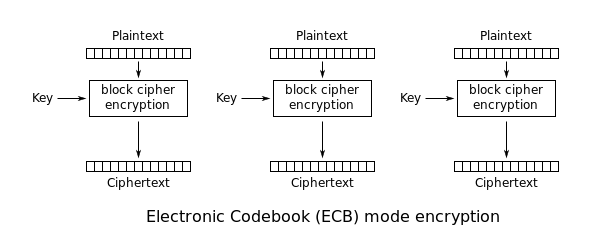
\includegraphics[height=0.15\textwidth]{res/ECB-ENC.png} 
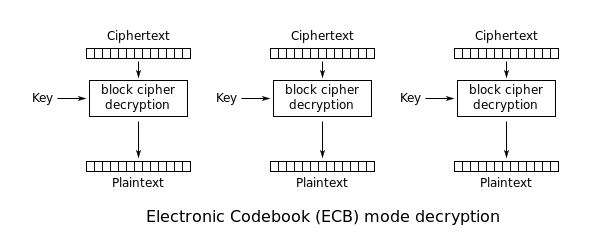
\includegraphics[height=0.15\textwidth]{res/ECB-DEC.png}
\end{center}
\item \textbf{Cipher Block Chaining}
\label{sec:org4854831}
This block cipher uses the concept of nonces (\emph{nonsense}) to add entropy to the cipher output. If the IV (nonce) isn't reused, CBC is IND-CPA. Note that although we can't parallelize the encryption, we can parallelize the decryption. The structure is the following:

\begin{align*}
C_0 &= IV \\
C_1 &= E_k(C_{i-1} \oplus P_i) \\
P_i &= D_k(C_i) \oplus C_{i-1}
\end{align*}

\begin{center}
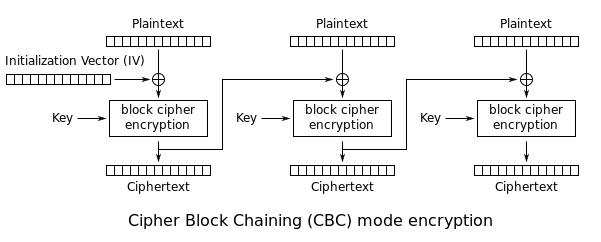
\includegraphics[height=0.15\textwidth]{res/CBC-ENC.png} 
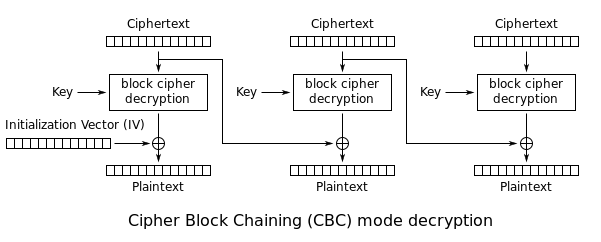
\includegraphics[height=0.15\textwidth]{res/CBC-DEC.png}
\end{center}
\item \textbf{Counter Mode}
\label{sec:orgcc295e4}
All-parallelizable alternative to CBC. Instead of one IV, uses \(nonce || i, i \in [0,...,n]\) with \emph{n} being the number of blocks. Reusing the IV in CBC makes it lose the IND-CPA game, but it's not catastrophic because the attacker will only find out the first block. If you reuse the IV in CTR mode, it transforms itself into the one time pad, leaking all the message. Note that CTR decryption uses the nonce encryption instead of a decryption function and that it is not exactly a block cypher but more of a stream cypher because it doesn't need padding. The structure is the following:

\begin{center}
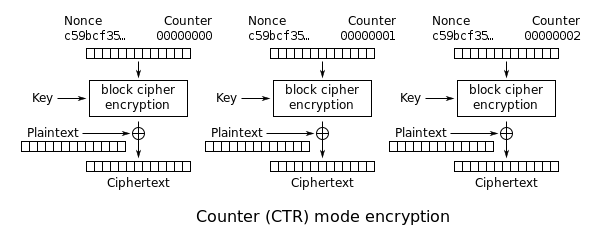
\includegraphics[height=0.15\textwidth]{res/CTR-ENC.png} 
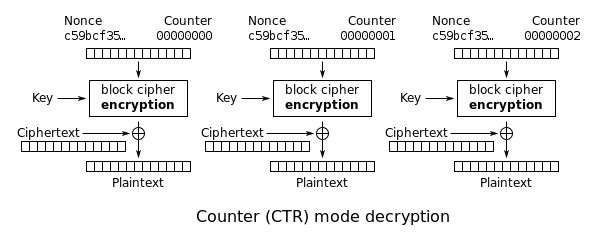
\includegraphics[height=0.15\textwidth]{res/CTR-DEC.png}
\end{center}
\end{enumerate}
\subsection{Hashes}
\label{sec:org38ebbcc}
Hash functions have the following:
\begin{itemize}
\item Variable input size
\item Fixed output size
\item Efficient computation
\item Pseudo-Random
\end{itemize}
Along with that, we must make sure that the hash functions provide us with these properties:
\begin{itemize}
\item One-way: easy to compute, almost impossible to revert the process.
\item Second Preimage resistant: given \emph{x}, almost impossible to find a \emph{x'} s.t. Hash(x) = Hash(x').
\item Collision resistant: Almost impossible to find x, y s.t. Hash(x) = Hash(y) (Collision resistance implies second preimage resistance)
\end{itemize}
\subsection{Message Authentication Codes}
\label{sec:orgacb8a3c}
MACs are checksums for messages, meaning they are sent with the message so that they are proven to be untampered. MACs, as encryption algorithms, need a key to be private only between the ones that are sharing the message. As an example:

\begin{align*}
   A &: C = E_{EK}(M) \\
   A &: T = MAC(MK, C) \\
   A &\to_{\{C, T\}}B \\
   B &: T = MAC(MK, C)?
\end{align*}

If the operation on the last line says that they are not equal, B can assume that the message has been tampered with. Also, the convention of using the MAC in the encrypted message is the correct way of using it since \textbf{MACs are deterministic and leak information}. \textbf{Never use the same key for MAC and Encryption}. 
\subsection{Password Storage}
\label{sec:org4889b8a}
Passwords should not be stored in a map \texttt{\textbackslash{}\{User, Password\textbackslash{}\}} because if someone gets ahold of this structure, they can simply impersonate everyone. We want the password to be a secret to our server. To do that we can store the map \texttt{\textbackslash{}\{User, Hash(Password)\textbackslash{}\}}. This way, if someone gets this information, they can't do much because of the \emph{One-way property} of hashes. The user would input the password and send the hash of it to the server, which would then check if it's correct.

However, many people choose poor passwords. Consider that the attacker knows what's the hash function by using the server as an oracle. \uline{What can he do with the fact that there are simple passwords scattered around many users?} He can create a brute forced dictionary with all the simple passwords and their hashes so that, when it gets ahold of the server's structure, it can just match the hashes with its dictionary (Dictionary Attack). We can mitigate that by adding a random, user-specific (unique) Salt (giant random number) to the user's password before it's hashed. This way, even if the attacker can get its hands on the hash, they will never match the weak password's. We also would like for the hashing process to be slow, which would make the brute forcing much slower.
\subsection{Pseudo Random Number Generators (PRNGs)}
\label{sec:org9ff997a}
A PRNG needs the following functions: \texttt{seed(x), reseed(x), generate(size, x=optional)}. The \emph{x} in the functions are the true sources of entropy. The PRNGs should be predictable only if you know its internal state and should be roll-back resistant, meaning their internal state at time \emph{T-1} should not be determinable by someone with the knowledge of the state at \emph{T}. 
\subsection{Asymmetric Encryption}
\label{sec:orgbd178c0}
Although symmetric encryption looked as if it had everything taken care of, we must understand how \emph{A} and \emph{B} shared the secret key \emph{K}. If they haven't met up in person to share it, it is very likely the key is not a secret. Let's look at some encryption algorithms that take care of this aspect.
\subsubsection{Diffie-Hellman}
\label{sec:orgcf06109}
\label{DH}
The event \emph{A} wants to communicate with \emph{B} follows this sequence of operations for \emph{p} (huge prime) and \emph{g}, \(1 < g < p - 1\) public. 

\begin{align*}
  A &: a \in \{0,1,...,p-2\} \\ 
    &: X_A = g^a \mod(p) \\
  B &: b \in \{0,1,...,p-2\} \\ 
    &: X_B = g^b \mod(p) \\
  A &: broadcast(X_A) \\
  B &: broadcast(X_B) \\
  A &: S = B^a \mod(p) = g^{ab} \mod(p) \\
  B &: S = A^b \mod(p) = g^{ab} \mod(p)
\end{align*}

Now that they have a symmetric key \emph{S}, they can simply use a symmetric encryption system. Have in mind that a man in the middle can read \(g^a\), \(g^b\) and \(g^{a+b}\) but can never get to \(g^{ab}\) because they don't know \emph{a} or \emph{b} and can't break the modular equation because that would require it to break the discrete log, which is extremely hard. However, a man in the middle can intercept the messages and just create its own \(X_M\) and \emph{m} to structure two different channels: one with \emph{A} and one with \emph{B}.
\subsubsection{El-gamal Encryption}
\label{sec:org701879f}
This algorithm uses a similar idea as \emph{Diffie-Hellman's}. We have all the information listed above. From that, we want \emph{A} to send a message to \emph{B} (the message must be \(\in \{1,...,p-1\}\)). We do:

\begin{align*}
  A &: r \in {0,...,p-2} \\
  A &: \{R, S\} = \{g^r \mod(p), M * X_B^r \mod(p)\} \\
  A &\to_C B \\
  B &: R^{-b}*S \equiv g^{-br}*M*X_B^{r} \equiv g^{-br}*M*g^{br }\equiv M \mod(p)
\end{align*}

We know that only \emph{B} can decrypt it because it is the only one that knows its private key \emph{b} and can compute \(R^{-b}\). We must not reuse \emph{r} or else it will leak information.
\subsubsection{RSA Encryption}
\label{sec:org3d8b1b1}
This one is definitely the most complicated one. \emph{A} generates two private primes \emph{p, g}; calculates public \(n=p*g\) and private \(\phi(n) = (p-1)(g-1)\); picks random public \(2 < e < \phi(n)\); solves private \(d = e^{-1} \mod(\phi(n))\). Now if \emph{B} wants to send a message to \emph{A}, this is how it goes:

\begin{align*}
  B &: C = M^e \mod(n) \\
  B &\to_{C }A \\
  A &: C^d \equiv M^{ed} \mod(n) \\
    &: ed \equiv 1 \mod (\phi(n)) \to ed - 1 = k\phi(n) \\
    &: M^ed \equiv (M^{\phi(n)})^k * M \equiv_{Euler_{thm}} 1^k * M \equiv M \mod (n)  
\end{align*}

However, the encryption is deterministic for the same \emph{e}, meaning it can leak information! There should be a source of entropy in it, but it isn't that important for our scope.

\subsection{DSA Signatures}
\label{sec:orgcb076f7}
Based on Diffie-Hellman. Signatures are used to avoid the man in the middle attack listed in \ref{DH}. Initial parameters: \texttt{L, N, Hash(x)}. \emph{A} creates an N-bit prime \emph{q}, L-bit prime \emph{p}, s.t. \(q|p\) and \(g = h^{\frac{p-1}{q} \mod(p), 1 < h < p-1\). We say \emph{p,g,q} are public. \emph{A} has the private key \emph{a} and the public key \(g^a \mod(p)\). \emph{A} calculates a random \(k < q\). And the process of signing by \emph{A} and verifying by \emph{B} goes as such:

\begin{align*}
 A &: r = (g^k \mod (p)) \mod (q), r \neq 0 \\
   &: s = k^{-1}(Hash(M) + ar) \mod (q) \\
   &: Sign = \{r, s\} \\
   &\to_{...||Sign} B \\
 B &: w = s^-1 \mod(q) \\
   &: u_1 = Hash(M) * w \mod (q) \\
   &: u_2 = rw \mod(q) \\
   &: v = (g^{u_1}g^{au_2} \mod(p))\mod(q)
\end{align*}

And if \(v = r\), the signature is valid!

\subsection{Certification and Authentication}
\label{sec:orge42dedf}
We trust a certificate authority, which gives us the correct certificate (public key) for whomever we want to speak to. The certificate should be signed by the CA itself or by someone the CA has signed a certificate to, meaning that it is trustworthy. The latter is the method for certification scaling, avoiding the bottleneck of having one CA authenticating numerous users and implementing a signature delegation (Hierarchical). We should also be able to receive a list of certificate revokations so we can avoid insecure connections. 

\section{Web Security}
\label{sec:orge0b6626}
This section will focus on the possible exploits and mitigation options for web pages as well as the structure of the web.
\subsection{SQL Injection}
\label{sec:org6189187}
This is probably the most known system attack these days. It's really simple to understand and avoid.

Web servers/pages can have databases. The most known Database Query language is SQL. Usually, the web server/page would have queries to fill out information on the HTML rendering and such. For this, they must, sometimes, read user input and add it as a field to the query code. \uline{You have a social media website. You want to display someone's profile when it is searched for. You create a field in the web page asking "Looking for\ldots{}?". The intended output of a query in this scenario would be all the users information (name, age, \ldots{}). So you add the following to your code:}

\begin{minted}[,bgcolor=yellow]{sql}
SELECT name, age, photo FROM users WHERE username = input; 
\end{minted}

\uline{What can an attacker do?} It can use a string like the following: \texttt{''; DROP TABLE users;-{}-}, which will end the query, break the line, add a \emph{drop table} command and comment whatever is in the right just to make sure. This will break the website.
The best mitigation for this are \emph{prepared statements}, which will send the input all the way to a leaf inside the tree structured query, taking away all its privileges of running any commands.
\subsection{Javascript \& Cookies}
\label{sec:orgabf6e93}
Javascript is a scripting lenaguage used to structure and add functionalities to your webpage. It can basically do whatever it wants to the \textbf{DOM} as well as read/change the session cookies. In order to make your computer safe from dangerous websites with Javascript that you may end up visiting, Javascript is \emph{sandboxed}, which means it cannot change files or programs in the computer it is being run on.
\subsubsection{Same-Origin Policy}
\label{sec:org001422d}
Another danger of Javascript is the fact that it should be able to tamper with other websites. That's why there is \textbf{SOP}. The policy restrains webpages from affect things that are out of their origin. For two origins to be the same, they must have the same \texttt{domain, port, protocol}. \uline{For example, the website \url{http://amazon.com/idk/1023} has the same origin as \url{http://amazon.com:80/babyyoda/1123421} but not of \url{https://amazon.com/idk/1023}, \url{http://store.amazon.com/idk/1023} or \url{http://amazon.com:1234/idk/1023}}.
\subsubsection{Cookies!}
\label{sec:org7ba8b5e}
Cookies are basically variables for someone's session in a website. They are structured with a \texttt{host, path} key and a value. This is how companies track what Ads you want to see. Here are some cookie properties:
\begin{enumerate}
\item \textbf{Cookie Origin Policy}
\label{sec:org4439d02}

\textbf{Don't confuse this with SOP!} Cookie origin policy restrains the cookie sharing process as in \emph{"which websites can receive my cookies"}. The only websites that can share your cookie are the ones that have matching suffixes. \uline{E.g. example.com/foo shares with www.example.com/foo but not with example.com/bar}. 
\item \textbf{Secure Flag}
\label{sec:org4b8d8e5}

A cookie can be set with a secure flag, which means it can only be sent via \emph{HTTPS} connection.
\item \textbf{HTTP-Only Flag}
\label{sec:org672fec9}

A cookie set with the HTTP-Only flag will only be accessible in the server side.
\end{enumerate}
\subsubsection{Spectre Attack}
\label{sec:org26f81c5}
A hardware side channel developed to access the nested iframe's information by treaking the processor's predictor. Solution is to make the browser \textbf{eat RAM} by giving every website it's own process.
\subsection{Cross-site Forgery Attack (CSRF)}
\label{sec:org94f94e7}
Attacker inserts malicious request in a page it has control inside an \texttt{<img>} tag or any other operation that causes the request to run. \uline{E.g. You visit the attacker's webpage, which files a transfer request in your name on www.bank.com. Is that going to work?}. It depends on how the bank implements its system. The point of this attack is to take advantage of the cookies saved for the victim. So if the bank determines who is logged in by the cookies, then the attack might work. There are two important mitigation options for this exploit:
\subsubsection{"Referer" validation}
\label{sec:org3376aad}
The "referer" validation allows the website to identify from which website the request is coming from. If the website is not itself, it makes sense to terminate the operation. However, there are still some ways of going around it.
\subsubsection{Secret Token Validation}
\label{sec:orgd4efbda}
A short TTL random cookie that defines the login session for the user. We can add this cookie to the URL, making the URL itself hold entropy, which means the attacker's only option is to brute force the cookie (probably infeasible) or find a way to retrieve it. The solution, however, is not really pretty and Weaver doesn't consider any solutions regarding the STV perfect, but it is better than the "referer" validation.

\subsection{Cross-site Scripting (XSS)}
\label{sec:org2e95d61}
Its main objective is to Subvert the SOP.
\subsubsection{Stored XSS}
\label{sec:org2be2a3a}
Persisting a malicious script (Javascript) in a server that's going to be accessed by the victim, running the code. In the end, it can either execute whatever malicious operation it wants in the website using the victims authentication cookie or it can send data (cookies mostly) to the evil server.
\subsubsection{Reflected XSS}
\label{sec:orgdc814a3}
User enters malicious website, clicks on a link that redirects him to a website whose cookies are interesting with a script in the URL. The script can either send data to the attacker or perform malicious operations in the name of the user.
\subsubsection{How to fix?}
\label{sec:org05c393b}
\begin{itemize}
\item Input sanitation (CSP) \(\to\) Removes whatever might be fishy about an input
\begin{itemize}
\item Prohibit inline scripts
\item Whitelisting
\item Blacklisting
\end{itemize}
\item HTTP-only flag \(\to\) doesn't allow the user to access its cookies, so the script can't get them.
\end{itemize}

\subsection{Clickjacking}
\label{sec:org4620887}
Placement of invisible i-frames of a target website over some enticing content or placement of visible of a target under a malicious invisible frame to capture user input. We can fix it by frame-busting: website prohibits its page from being a frame or by using the HTTP \textbf{X-Frame-Options}, which whitelists some websites for frame use. 

\section{Network Security}
\label{sec:orge0c3ef6}
This is most certainly the hardest part of the content. This is an overview for Networking as well as an observation set for its vulnerabilities.
\subsection{The 5 layers that actually matter}
\label{sec:org9db5d57}
We can divide networking into 5 different layers, the lowest their number, the lower levelled they are. These are:

\begin{center}
\begin{tabular}{r|l|l}
\hline
7 & Application & Communication of whatever (e-mail, torrent,\ldots{})\\
\hline
4 & Transport & End-to-end communication between processes (TCP/UDP)\\
\hline
3 & (inter)Network & Bridges multiple "subnets" to provide end-to-end connectivity\\
\hline
2 & Link & Framing and transmission of bits into a message\\
\hline
1 & Physical & Encoding bits to send them over a link (single)\\
\hline
\end{tabular}
\end{center}
\subsection{Basic stuff}
\label{sec:orgbb0ef21}
\begin{itemize}
\item IPv4 \(\to\) 32-bits
\item IPv6 \(\to\) 64-bits
\item localhost \(\to\) 127.0.0/24
\item Broadcast \(\to\) 255.255.255.255
\item Protocols \(\to\) agreement on how to communicate (Format, order of message, etc.)
\item Packets \(\to\) What communication is broke into
\begin{itemize}
\item Software doesn't see it;
\item May be dropped;
\end{itemize}
\item Attacker types:
\begin{itemize}
\item Off-Path Attacker: Can't see the victim's traffic;
\item On-Path Attacker: Can see the victim's traffic and add packets with race condition;
\item In-Path Attacker: Can see the victim's traffic, add packets without race conditions and drop packets.
\end{itemize}
\end{itemize}

\subsection{Local Network Connection}
\label{sec:org4d501d8}
When connecting to a network, a device needs to receive a configuration (IP Addr., Gateway and DNS Addr.) from some other system inside a network. 

\subsubsection{DHCP (Dynamic Host Control Protocol)}
\label{sec:orgc578e1e}
To receive the configuration, our host will broadcast a \emph{Server-Discovery} message that will be answered by the \textbf{DHCP} server of the network. The answer will consist of an offer which our host will accept or not and communicate to the server, that will ACKnowledge it. The offer has all the configuration needed.

If someone hears the broadcast and sends an offer before he DHCP server, it could result in big trouble since they can redirect us to any DNS and Gateway of their choosing, meaning our connection has been completely hijacked and they have full control of what we are looking for and at. We now have a complete Man in the Middle. This scenario is called the \emph{Rogue Access point}.

\subsubsection{ARP}
\label{sec:org2f2c47f}
The Link can't see the IP Addr. and that's why we need a MAC address for communication. the \textbf{ARP} protocol is to whom we will turn we need to find another device. We send its IP and:
\begin{itemize}
\item If the IP is in the local network \(\to\) receive its MAC;
\item Else \(\to\) redirects us to the Gateway, to whom we will send our packets in order to get routed towards the destination;
\end{itemize}

\subsubsection{\emph{AirPwn}}
\label{sec:orgc077b8f}
When the traffic is non-encrypted and the attacker knows to whom the traffic belongs, it can inject packets, meaning they can race the server to which the client is connected for a response. If the attacker wins, the client receives its malicious packets.

\subsubsection{WPA2}
\label{sec:org499e756}
The WPA2 execution works as the followin sequence of events (C \(\to\) client, AC \(\to\) Access Point, F \(\to\) Key derivation function):

\begin{align*}
 C,AC &: PSK = F(passwd||SSID) \\
 AC &: Anonce = generate() \\
 C &: Snonce = generate() \\
 AC &\to_{Anonce }C \\
 C &: PTK = F(PSK, Anonce, Snonce, MAC_AP, MAC_C) \\
 C &\to_{Snonce||MIC} AC \\
 AC &: PTK = F(PSK, Anonce, Snonce, MAC_AP, MAC_C) \\
 AC &\to_{GTK||MIC} C \\
 C &\to_{ACK}_{} AC
\end{align*}

Now both devices have the symmetric PTK (Pairwise Transient Key)! Although all the communication between \emph{C} and \emph{AC} can be encrypted from now on, this doesn't prevent someone that has the password from deriving the key if it knows the MAC of the client because the attacker would be able to see all the rest! Even if it doesn't know the PSK, it can still try to brute-force it. This isn't a really safe protocol.

\subsubsection{WPA2 Enterprise}
\label{sec:org58239c7}
WPA2 Enterprise is different. It is much better. The 4-way handshake now happens between the device and an Authentication Server that holds the information required for each user, i.e. each user has an username and a password. This idea makes it so that if someone has access to the internet, it has its own PSK. So, even if the attacker had access to the internet, it wouldn't be able to understand someone else's 4-way handshake. Also, the Authentication Server's connection is encrypted with public-key encryption.

\subsubsection{LAN Security}
\label{sec:orgb4d0385}
Either we don't provide or we do some \emph{smart switching} and \emph{active monitoring}. 
\begin{enumerate}
\item \textbf{Switch}
\label{sec:orgd87f2db}

The Switch keeps track of where the MAC addresses inside the local network are seen in order to make things more efficient.
\item \textbf{VLANs}
\label{sec:orga426a11}

VLANs are smarter switches. They isolate different parts of the network, making all network traffic inside a VLAN stay inside it.
\end{enumerate}
\subsection{Transport Protocols}
\label{sec:org648dde9}
Before we get into actual communication between IPs and connection resolution for those, we need to clear up what are the transportation protocols for messages and how they work in a pretty abstract way.
\subsubsection{UDP (User Datagram Protocol)}
\label{sec:org9a65c71}
Also called "Unreliable" Datagram Protocol, UDP is a lightweight datagram transportation protocol that relies itself in a \emph{best effort} execution, meaning packets can be dropped or arrive in a different and it won't care. Now this clearly seems a really bad way to send a message. The point is: \textbf{It is really efficient}.
\subsubsection{TCP (Transmission Control Protocol)}
\label{sec:org13ac913}
The TCP usual communication between two entities are set and terminated goes as the image \ref{tcp} shows us. Once the communication is set, we can start sending and receiving data. As shown, the connection starts with a Sequence Number from the client as well as another one from the server. The acknowledgment field is always sent as the received Sequence Number plus the amount of data (flag packets are sized one) received and the Sequence Number is always sent as the previous received ACK. The same will happen on data transferring.  

\begin{figure}[htbp]
\centering
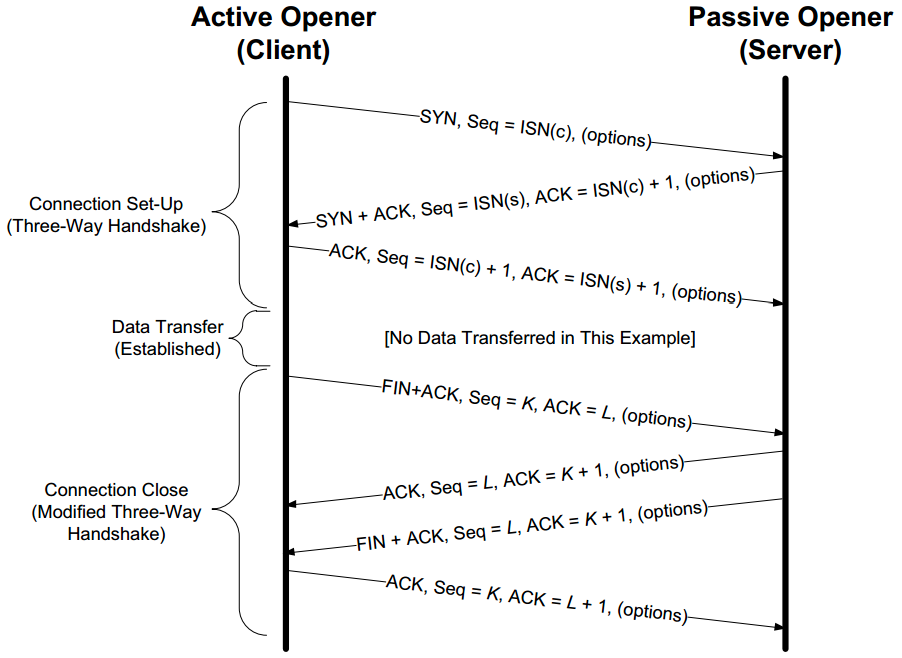
\includegraphics[height=0.5\textwidth]{res/TCP.png}
\caption{\label{tcp}
TCP execution}
\end{figure} 

\subsubsection{Flags}
\label{sec:orgff72e27}
It's also important to understand what the packet flags mean.
\begin{itemize}
\item SYN \(\to\) Initiate connection;
\item ACK \(\to\) Acknowledge message arrival;
\item FIN \(\to\) Warn that data won't be sent anymore, but the channel is still open for receiving;
\item RST \(\to\) Terminate connection \(\to\) \textbf{Something went wrong!}
\end{itemize}
\subsubsection{Packet \& RST Injection}
\label{sec:orgdafbab6}
Also, someone who can see the TCP traffic can inject packages. Someone who doesn't can guess the port and Sequence Number. A "RST" packet doesn't need any Sequence Number, so if someone knows the target IP and can guess the port, it can just terminate a connection.
\subsubsection{SYN Flooding!}
\label{sec:orgac9980e}
SYN Packets allocate state inside the server. Spamming SYN requests can cause Denial of service. To fix this, we need \textbf{SYN Cookies!} The idea behind it is to send a random generated number as the sequence number to the client so that the client has to send it back to you before you actually allocate state. However, we need to assert that the number is the same. For this, we use HMAC. We allocate space, but it's much less than before. The space allocated is for the number we input in the HMAC function. This way we send HMAC(k) and check if the return \emph{x} provides us with HMAC(x) = HMAC(k).  
\subsection{DNS}
\label{sec:org6643c62}
Finds an IP Addr. for communication based on a given URL. Uses UDP because it's performance critical. It's considered a distributed database in which the DNS resolver asks each Name Server for the URL's existance.
\subsubsection{DNS Resolver}
\label{sec:org5d5ad7b}
The DNS Resolver can be Reursive or Iterative. \uline{Recursive}: Local DNS server \(\to\) Root (.) \(\to\) following name server \(\to\) \ldots{}; \uline{Iterative}: Local DNS server looks for Root, that returns the following name server, and then looks for the name server\ldots{}
\subsubsection{DNS Response}
\label{sec:org6947433}
The DNS Response has the following structure:

\begin{center}
\begin{tabular}{l|l}
\hline
Question & Request\\
\hline
Transaction ID & Identification\\
\hline
Answer & If there is any, the requested IP\\
\hline
Authority Section & Name Servers responsible for the answer or the following lookups\\
\hline
Additional Section & Useful info to be cached (possible following lookups)\\
\hline
\end{tabular}
\end{center}

All sections besides "Transaction ID" are consisted by Resource Records. RRs are structures that contain the following values:
\begin{itemize}
\item Hostname \(\to\) The hostname it represents;
\item TTL \(\to\) Time to live;
\item Family \(\to\) Always going to be "IN" (Internet);
\item Type \(\to\) Type for the value:
\begin{itemize}
\item NS \(\to\) Name Server;
\item A \(\to\) IPv4 Addr;
\item AAAA \(\to\) IPv6 Addr;
\end{itemize}
\item Value \(\to\) The value it holds
\end{itemize}
\subsubsection{Bailiwick Check}
\label{sec:orgc61f063}
Name server can't add names in the Additional or Authority section for names that aren't in bailiwick, meaning they aren't part of the lookup host. This is to avoid that the Name Server for "mit.edu" adds "berkeley.edu" to the Additional Section with some malicious IP address when someone looks it up. E.g. if you are looking up "eecs.mit.edu" only accept from "\textbf{*}.mit.edu".
\subsubsection{Blind Spoofing}
\label{sec:org77ef76a}
This attack involves having someone in a malicious webpage or having them click some bait so that they try to access a specific website, say "bank.com". Once they run the DNS query, the attacker is going to try running against the server response so it may be able to poison the user's DNS cache. To do this, the attacker must be able to spoof the transaction ID, which is random. If it succeeds, the user may have a malicious website instead of "bank.com" and so it goes. 
\subsubsection{The Kaminsky Attack}
\label{sec:org41108b0}
Although the idea above seems doable, it's really hard to actually make anything out of it. Consider that you have only one chance of succeeding. Once the value of the lookup is cached, there is nothing we can do about it but wait its TTL. The Kaminsky Attack is a well elaborated alternative to the blind spoofing. In spite of it actually doing mostly the same thing (guessing ID and trying to run), this method, instead of running the lookup to the actual website, looks up fake websites such as "a.bank.com", "b.bank.com",\ldots{}; Websites that are in Bailiwick and that aren't cached. This way, it still only caches the value when it guesses the correct ID and wins the race, but it can try that as many times as it wants! Some techniques to avoid that is to add CaMeLcAsE letters in the Name Servers and randomize the source port. These two options make spoofing much harder, but still very possible.

\subsection{TLS}
\label{sec:org381965f}
Built on top of TCP, TLS uses the same ACK/SEQ behaviour. The process is shown by \ref{TLS} \sout{With some english mistakes but I found that on Google Images so I don't care}. As we can see, the handshake happens by them agreeing on a Cipher spec available for one of the Client's Crypto options. Each one also sends a random 256-bit number (R\textsubscript{C}, R\textsubscript{S}) to add entropy and avoid replay attacks (isn't shown on image though). The server also sends its certificate for the client to authenticate and start the key sharing process. When the key exchange is done, the data will be communicated in the following format: \(\{M,MAC(I, M)\}_C\). Each entity will have its own Cipher and Integrity key to avoid replay attacks with same Sequence Numbers. The key exchange, however, isn't tackled in depth. For that, let's keep going.

\begin{figure}[htbp]
\centering
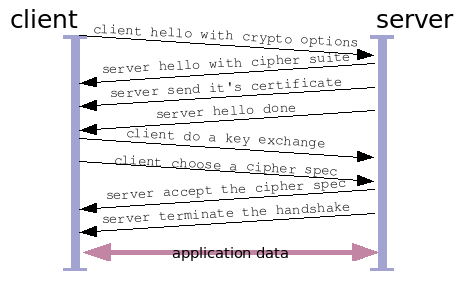
\includegraphics[height=0.5\textwidth]{res/TLS.png}
\caption{\label{TLS}
TLS Behaviour}
\end{figure}

\subsubsection{TLS with Diffie-Hellman}
\label{sec:orge8b7ede}
Once having its certificate authenticated by the client, the server sends \(\{g,p,g^a \mod(p)\}_{K_{server}^{-1}}\). Once the client receives this, the server sends a "end of handshake" message as the client sends \(g^b \mod(p)\). Now they both have the \emph{PS} and can derive \(C_C, C_S\) (cipher keys) and \(I_C, I_S\) (Integrity keys) from \{PS, R\textsubscript{C}, R\textsubscript{S}\}. Having all keys, they MAC and send the whole handshake using the Integrity keys to make sure they were derived correctly. Using DH provides forward secrecy, which means that if someone gets ahold of the client or the server's private key in the future, they wouldn't be able to understand the dialog since \emph{a} and \emph{b} were deleted when the conversation stopped.
\subsubsection{TLS with RSA Encryption}
\label{sec:orga3757ec}
The difference is that, instead of sending a generated DH public key with its certificate, the server waits for the client to send \(\{PS\}_{K_{server}}\) and then all goes along the same way. 
\subsection{{\bfseries\sffamily TODO} Certificate Authorities - Revised}
\label{sec:orgc5bede1}
\subsection{{\bfseries\sffamily TODO} DNSSEC}
\label{sec:org3b73afc}

\section{Appendix}
\label{sec:org25e44fc}
\subsection{Assembly code for Immediate suffering}
\label{sec:orga24d240}
\label{sec:Assemble}
Let's review some topics for the Assembly code structure when generated through C code.
\subsubsection{Registers}
\label{sec:org3694198}
For the purpose of this class, I'm sure we'll only need to know 32-bit registers (not that there are many differences between 32 to 64, but the names differ).
\begin{itemize}
\item Data registers \cite{evans_guide_nodate}:
\begin{itemize}
\item \textbf{EAX} \(\to\) Accumulator: IO and Arithmetic functions, \textbf{Is where the return value is stored};
\item \textbf{EBX} \(\to\) Base: Indexed addressing;
\item \textbf{ECX} \(\to\) Count: Loops
\item \textbf{EDX} \(\to\) Data: Basically the same as \textbf{EAX};
\end{itemize}
\item \hyperref[StackReg]{Pointer registers}
\begin{itemize}
\item \textbf{EBP} \(\to\) Base: Holds the base address for the stack;
\item \textbf{ESP} \(\to\) Stack: Holds the top address for the stack;
\item \textbf{EIP} \(\to\) Index/Instruction: Holds the offset for the next instruction
\end{itemize}
\end{itemize}

\begin{figure}[htbp]
\centering
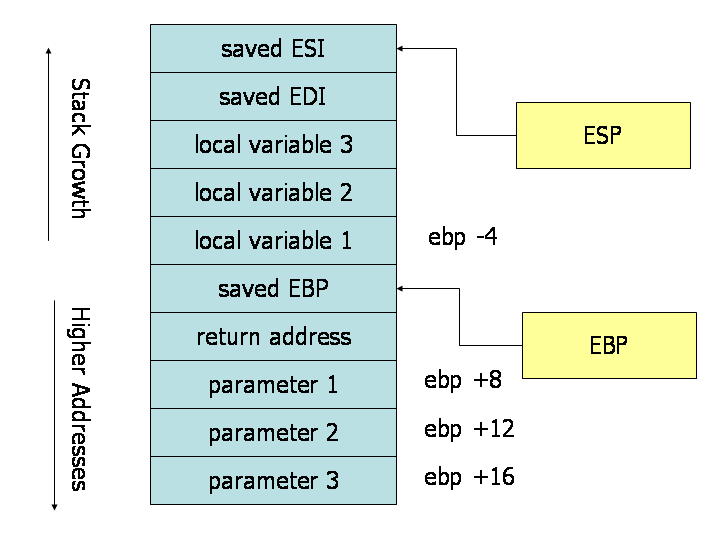
\includegraphics[width=3in]{res/stack-convention.png}
\caption{\label{StackReg}
The Stack registers layout}
\end{figure}

\subsubsection{How do function calls work?}
\label{sec:org88a9049}
This part is really important for us so we actually understand how the stack layouts itself on \emph{return} and exploit the return address. It follows these operations \cite{hu_understanding_nodate}:

\begin{itemize}
\item Setup \& execution
\begin{itemize}
\item Push all the function parameters into the stack (piles up from last to first \(\to\) first one in the lowest memory address);
\item Call the function by running \texttt{call};
\item Push the \emph{Return Address} into the stack;
\item Points \texttt{EIP} to the start of the function;
\item Save the previous \texttt{EBP} on top of the stack;
\item Set \texttt{EBP} and \texttt{ESP} to point to the value of the old \texttt{EBP} (top of the stack, which means \texttt{ESP} was already pointing at it);
\item Stack the \texttt{callee registers};
\item As the local variables are declared, we decrease the value of \texttt{ESP} to increase the size of the stack frame;
\end{itemize}
\item Return 
\begin{itemize}
\item Store the return value in \texttt{EAX};
\item Pop the \texttt{callee registers};
\item Make \texttt{ESP} equal \texttt{EBP};
\item Pop the old \texttt{EBP} to \texttt{EBP} (\texttt{pop ebp}, \texttt{ESP} will increase value because the stack size gets smaller);
\item As \texttt{ESP} now points to the \emph{return address} (which was stored right on top of \texttt{EBP}), \texttt{ret} will make the \texttt{EIP} point to the correct address.
\end{itemize}
\end{itemize}

\subsection{Variable Layout in the Stack}
\label{sec:org126d5dc}
\label{sec:VarLayoutStack}
We have some important fields and their data size. Their data size is the amount of space they occupy in the Stack, Heap, etc. These are:

\begin{center}
\begin{tabular}{l|l}
\hline
int & 4 bytes\\
\hline
float & 4 bytes\\
\hline
double & 8 bytes\\
\hline
char & 1 byte\\
\hline
\end{tabular}
\end{center}

Consider that \texttt{long, short} usually increase and decrease, respectively, around \texttt{4 bytes}.

For structures, however, we have a more complex layout. The first declared variable will be in the lowest memory position and the last one in the highest. The following example shows the Stack layout once we declare a structure variable:

\begin{minted}[]{c}
typedef struct {
  int i;
  char c;
  float f;
  double d;
} Sample;

int main() {
  Sample sample = {1, '2', 3.0, 4.0};
  return 0;
}
\end{minted}

Given this code, once we execute \texttt{main}, we'll have the following structure in the Stack:

\begin{center}
\begin{tabular}{l|l|l}
\hline
LOWEST Memory Addr. & ESP & 4 bytes\\
\hline
 & sample.i & 4 bytes\\
\hline
 & sample.c & 1 byte\\
\hline
 & sample.f & 4 bytes\\
\hline
 & sample.d & 4 bytes\\
\hline
 & EBP & 4 bytes\\
\hline
HIGHEST Memory Addr. & return address & 4 bytes\\
\hline
\end{tabular}
\end{center}




\subsection{{\bfseries\sffamily TODO} Using GDB \& Shell Exploits}
\label{sec:org046a466}
\subsection{{\bfseries\sffamily TODO} Nick's Insane way of Checking a Lie}
\label{sec:org06d43a7}


\bibliographystyle{unsrt}
\bibliography{CS_161_Summary}
\end{document}
